\documentclass[]{standalone}

\usepackage{tikz}
\usetikzlibrary{automata, positioning, arrows}

\begin{document}
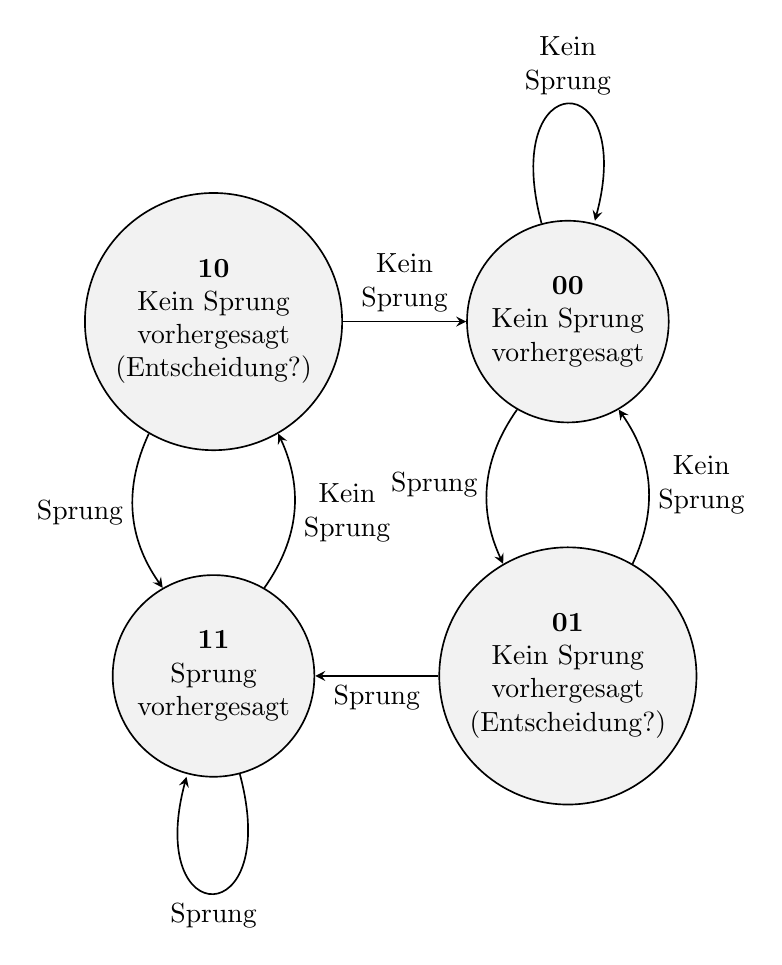
\begin{tikzpicture}[node distance=4.5cm]
	\tikzstyle{every state}=[semithick, fill=gray!10]
	\tikzstyle{every edge}=[draw,->,>=stealth,auto,semithick]

	\node[state,align=center] (11) {\textbf{11}\\Sprung\\vorhergesagt};
	\node[state,align=center,above of=11] (10) {\textbf{10}\\Kein Sprung\\vorhergesagt\\(Entscheidung?)};
	\node[state,align=center,right of=11] (01) {\textbf{01}\\Kein Sprung\\vorhergesagt\\(Entscheidung?)};
	\node[state,align=center,above of=01] (00) {\textbf{00}\\Kein Sprung\\vorhergesagt};

	\draw (00) edge[bend right,left] node {Sprung} (01)
	edge[loop above] node[align=center] {Kein\\Sprung} (00);
	\draw (01) edge[bend right,right] node[align=center] {Kein\\Sprung} (00)
	edge node {Sprung} (11);
	\draw (10) edge[bend right,left] node {Sprung} (11)
	edge node[align=center] {Kein\\Sprung} (00);
	\draw (11) edge[bend right,right] node[align=center] {Kein\\Sprung} (10)
	edge[loop below] node {Sprung} (11);
\end{tikzpicture}
\end{document}
